%%%%%%%%%%%%%%%%%%%%%%%%%%%%%%%%%%%%%%%%%%%%%%%%%%%%%%%%%%%%%%%%%%%%%%%%%%%%
% AGUJournalTemplate.tex: this template file is for articles formatted with LaTeX
%
% This file includes commands and instructions
% given in the order necessary to produce a final output that will
% satisfy AGU requirements, including customized APA reference formatting.
%
% You may copy this file and give it 
% article name, and enter your text.
%
%
% Step 1: Set the \documentclass
%
%

%% To submit your paper:
\documentclass[draft]{agujournal2019}
\usepackage{url} %this package should fix any errors with URLs in refs.
\usepackage{lineno}
\usepackage[inline]{trackchanges} %for better track changes. finalnew option will compile document with changes incorporated.
\usepackage{soul}
\graphicspath{ {./figures/} }
\linenumbers
%%%%%%%
% As of 2018 we recommend use of the TrackChanges package to mark revisions.
% The trackchanges package adds five new LaTeX commands:
%
%  \note[editor]{The note}
%  \annote[editor]{Text to annotate}{The note}
%  \add[editor]{Text to add}
%  \remove[editor]{Text to remove}
%  \change[editor]{Text to remove}{Text to add}
%
% complete documentation is here: http://trackchanges.sourceforge.net/
%%%%%%%

\draftfalse

\journalname{Water Resources Research}


\begin{document}

%% ------------------------------------------------------------------------ %%
%  Title
%
% (A title should be specific, informative, and brief. Use
% abbreviations only if they are defined in the abstract. Titles that
% start with general keywords then specific terms are optimized in
% searches)
%
%% ------------------------------------------------------------------------ %%

\title{Green Infrastructure Placement Strategy in Urban Stormwater Network}

%% ------------------------------------------------------------------------ %%
%
%  AUTHORS AND AFFILIATIONS
%
%% ------------------------------------------------------------------------ %%

% Authors are individuals who have significantly contributed to the
% research and preparation of the article. Group authors are allowed, if
% each author in the group is separately identified in an appendix.)

% List authors by first name or initial followed by last name and
% separated by commas. Use \affil{} to number affiliations, and
% \thanks{} for author notes.
% Additional author notes should be indicated with \thanks{} (for
% example, for current addresses).

% Example: \authors{A. B. Author\affil{1}\thanks{Current address, Antartica}, B. C. Author\affil{2,3}, and D. E.
% Author\affil{3,4}\thanks{Also funded by Monsanto.}}

\authors{Xiating Chen\affil{1,2}, Xue Feng\affil{1,2}}

\affiliation{1}{Department of Civil, Environmental, and Geo-Engineering, University of Minnesota Twin Cities, Minneapolis, MN, USA}
\affiliation{2}{Saint Anthony Falls Laboratory, University of Minnesota Twin Cities, Minneapolis, MN, USA}

%(repeat as many times as is necessary)

%% Corresponding Author:
% Corresponding author mailing address and e-mail address:

% (include name and email addresses of the corresponding author.  More
% than one corresponding author is allowed in this LaTeX file and for
% publication; but only one corresponding author is allowed in our
% editorial system.)

% Example: \correspondingauthor{First and Last Name}{email@address.edu}

\correspondingauthor{Xiating Chen}{chen7090@umn.edu}

%% Keypoints, final entry on title page.

%  List up to three key points (at least one is required)
%  Key Points summarize the main points and conclusions of the article
%  Each must be 140 characters or fewer with no special characters or punctuation and must be complete sentences

% Example:
% \begin{keypoints}
% \item	List up to three key points (at least one is required)
% \item	Key Points summarize the main points and conclusions of the article
% \item	Each must be 140 characters or fewer with no special characters or punctuation and must be complete sentences
% \end{keypoints}

\begin{keypoints}
\item Urban stormwater network structure modulates green infrastructure effectiveness.
\item Tradeoff exists between hydrological outcomes, such as managing peak flow rate and inland flooding.
\item Effect of green infrastructure saturates at high rainfall intensity. 
\end{keypoints}

%% ------------------------------------------------------------------------ %%
%
%  ABSTRACT and PLAIN LANGUAGE SUMMARY
%
% A good Abstract will begin with a short description of the problem
% being addressed, briefly describe the new data or analyses, then
% briefly states the main conclusion(s) and how they are supported and
% uncertainties.

% The Plain Language Summary should be written for a broad audience,
% including journalists and the science-interested public, that will not have 
% a background in your field.
%
% A Plain Language Summary is required in GRL, JGR: Planets, JGR: Biogeosciences,
% JGR: Oceans, G-Cubed, Reviews of Geophysics, and JAMES.
% see http://sharingscience.agu.org/creating-plain-language-summary/)
%
%% ------------------------------------------------------------------------ %%

%% \begin{abstract} starts the second page

\begin{abstract}
%Runoff increases as a result of urbanization. Stormwater networks were built as a way to quickly transport runoff. They reduce inland flooding while resulting in higher peak flow downstream and in loss of groundwater recharge (the magnitude depends on the land and network configurations). As a counter-method, natural based solutions were implemented as a way to reduce runoff entering the USNs and partially restore the infiltration capacity to pre-development level. Currently literature on the interaction between USNs and GIs are limited; we want to investigate the aggregate effects of green infrastructure at a larger scale, beyond the confines of its site.  
%
%[ enter your Abstract here ]
Green infrastructure are nature-based solutions implemented to improve urban stormwater quality and reduce flooding. Currently, green infrastructure projects are implemented on a case-by-case basis, without considering their spatial configurations relative to each other or placement within the greater watershed. Here, we examine the optimal placement of green infrastructure sites within the urban drainage network -- which consist of grey infrastructure and mixed land use and land cover types -- to achieve the most flood control benefits. In our approach, we also explore the variabilities in design parameters and address the effects of climate uncertainty on green infrastructure performance.

To do so, we stochastically generate synthetic stormwater drainage networks on a square lattice, whose probability of occurrence follows a Gibbs’ distribution with a single parameter describing the sinuosity of the network. Then, different percentages of green infrastructure nodes representing green infrastructure sites are randomly placed across the network. The effects of network structure as well as green infrastructure coverage and  placement are investigated using EPA’s Storm Water Management Model (SWMM). To account for uncertainty in future precipitation patterns, we force the model with two-hour storms with return periods ranging from two years to 100 years. To account for the variability in the design and site parameters, we simulate our results using multiple parameter combinations based on user-submitted design and field measured data from the International Best Management Practice (BMP) Database. 

We find that there is no ``one-and-done” solution for green infrastructure planning. The structure of stormwater network alone, without green infrastructure, can modulate the peak flow rate and flood volume by changing the travel time in the network. When rainfall intensity is low, adding green infrastructure and placing them near the drainage outlet can most effectively reduce peak flow at the outlet. However, at higher rainfall intensities, green infrastructure can be overwhelmed and become ineffective at controlling flow. We anticipate that these results will serve as theoretical guidelines for optimal nature-based green infrastructure planning at the watershed scale.


\end{abstract}

\section*{Plain Language Summary}
[ enter your Plain Language Summary here or delete this section]


%% ------------------------------------------------------------------------ %%
%
%  TEXT
%
%% ------------------------------------------------------------------------ %%

%%% Suggested section heads:
% \section{Introduction}
%
% The main text should start with an introduction. Except for short
% manuscripts (such as comments and replies), the text should be divided
% into sections, each with its own heading.

% Headings should be sentence fragments and do not begin with a
% lowercase letter or number. Examples of good headings are:

% \section{Materials and Methods}
% Here is text on Materials and Methods.
%
% \subsection{A descriptive heading about methods}
% More about Methods.
%
% \section{Data} (Or section title might be a descriptive heading about data)
%
% \section{Results} (Or section title might be a descriptive heading about the
% results)
%
% \section{Conclusions}

\section{Introduction}

%What is runoff and how is it generated? 
%Why are we reducing runoff? 
%How are we reducing runoff? 
%- USNs 
%- Green infrastructure
%Scaling problem: Background on the interactions between green infrastructure and USNs, or Green infrastructure at different scales. 

%The increase of runoff due to land cover changes and urbanization has been well documented and studied for decades, and engineering solutions, ranging from the traditional storm sewers to stormwater best management practices (BMP) to green infrastructure (GI), have been mitigating flooding in urban watersheds. In general, impervious area reduces infiltration entering the soil and groundwater table, and increases direct runoff to storm sewers and streams \cite{Leopold1968}, although ongoing research to improve accurate runoff accounting continues. Some of the research advances our understanding in the nuances of effective impervious area \cite{Ebrahimian2016}, effective drainage area \cite{Miles2015}, and the impacts of construction related activities on soil composition in urban areas \cite{Gregory2006}. 

The increase of runoff due to the loss of infiltration capacity in urban landscape has been well documented and studied for decades. Underground stormwater drainage networks have been the standard practice to reduce inland flooding for over a century. Runoff from precipitation and snowmelt is quickly transported from upstream urban neighborhoods and discharged to downstream water bodies. These networks transform the stormwater watershed characteristics by shortening the lead and lag time of peak flow in urban streams, and they therefore contribute to higher peak flow during a storm event \cite{Graf1977, Jovanovic2019}. The magnitude of this increase in peak flow depends on the travel path configuration within the network \cite{Seo2012} and the geographical constraints of the landscape \cite{}. 

Concerned about peak flow increase and base flow decrease disrupting the receiving streams, engineers and planners have been designing and implementing green infrastructure to reduce runoff at source upstream. Green infrastructure (GI), also known as nature-based solutions and low-impact developments, is both small and large-scaled construction consisting of vegetation and soil (e.g., bio-retention cells, rain gardens, urban greeneries). Green infrastructure decreases the amount of runoff entering the stormwater networks by increasing infiltration and evapotranspiration, and at the same time, it naturally treats stormwater and recharges groundwater \cite{}(United States Environmental Protection Agency, 2020). The existing research focuses on both the technology advancement -- in the modeling and measurement of infiltration and pollutant transport phenomena in different porous media \cite{Xu2016, Zhang2018} -- and the feasibility and effectiveness of existing green infrastructure \cite{Avellaneda2017} at both small, household scale and large, municipal scale. However, the current implementations of green infrastructure are often limited to a parcel scale and primarily driven by stakeholder’s interests and convenience, and the design relies on the geographical factors of the project site \cite{}(Center for Watershed Protection; \& Maryland Department of the Environment, 2000). When a series of green infrastructure are retrofitted to the existing stormwater network, the spatial distribution of these sites in relation to the existing network becomes nontrivial. But there is very little understanding of the interaction between above-ground green infrastructure and below-ground pipe network. We want to investigate whether the placement of green infrastructure in a stormwater network can maximize hydrological benefits in an urban watershed. 

%both to attenuate peak flow and to allow for water-quality-related settling, stormwater BMP such as retention ponds have been either retrofitted and installed in municipal networks. However, some studies have suggested that stormwater BMP may have increased flashiness in outflow in arid climates \cite{McPhillips2019}, and they may unintentionally contribute to eutrophication downstream \cite{Taguchi2020}. 

%Urban stormwater runoff also has different biogeochemical composition from undeveloped headwater, and there are growing concerns around urban pollutants and nutrients contaminating the downstream waterbodies \cite{Finlay2011, Kaushal2012}. Road salts and washed-off car grease can enter natural stream via stormwater system as nonpoint source pollution. Meanwhile, trees, yard wastes, residential fertilizers and streets contribute to largely to the suburban residential nutrient budgets \cite{Bratt2017, Hobbie2017, Janke2017}. Unfiltered, untreated pollutant-containing stormwater runoff may also enter groundwater through leaky joints in aging infrastructure, and introduce a vertical dimension of challenges in urban water quality \cite{Kaushal2012}. 

In order to better integrate green infrastructure at a watershed scale, we use tools from graph theory to study and reconstruct the configuration of the urban stormwater networks. These complex infrastructure networks can be stripped down to their most basic components -- nodes and edges -- which store essential attributes for stormwater modeling. \textcolor{red}{Repeat definitions of nodes and edges.} This simplified configurations allow researchers to bypass the acquisition of infrastructure data, and to flexibly manipulate stormwater networks for scenario planning purposes while retaining their essential network structures. \textcolor{red}{Graph theories are sometimes referred to as network theories.} The field of network science studies how the components are connected, and how the structures influence the physical phenomena observed in the network \cite{Newman2010}. Originated from social network studies, networks and network theories have been applied in geosciences \cite{Heckmann2015} and ecology \cite{Carraro2020} to provide a perspective on large scale patterns that go unnoticed when focused on the individual parts. When these systems are translated to networks, one can compute the network properties, such as shortest paths between two nodes, or centrality indicators that can indicate the most important nodes within a graph. 

The existing network theory applications to hydrology include municipal and river networks generation \cite{Barnes2020, Poulter2008, Troutman1985, Troutman 1989, Seo2012, Seo2013}, network structural or scale-depent effects on hydrological responses \cite{Riasi2017, Rodriguez-Iturbe1979}, and optimization to improve hydrological network efficiency \cite{}. Tools from network theory are particularly helpful in understanding these hydrological pathways. They can generalize spatial layouts, demonstrate network properties without relying on the exact layouts, and still preserve the instantaneous unit hydrographs from observed stream flow data \cite{Seo2012}. In particular, the exact configurations of municipal stormwater networks exist as as-builts and shapefiles in municipal databases, and they are difficult to access due to geospatial data sharing restrictions. To overcome this challenge, we stochastically generate synthetic drainage networks, which probability of occurrence follows a Gibbs' distribution, to imitate a drainage network in a small urban catchment. 

\textcolor{red}{This should be an overview of the workflow. May flow better as a beginning paragraph for Methods section.} We want to establish a green infrastructure placement strategy at a watershed level and to upscale green infrastructure's effect on stormwater. To do so, we stochastically generate stormwater networks and model their hydrological responses with different numbers and locations of green infrastructure under a range of light to heavy rainfall scenarios. We hypothesize that green infrastructure performance depends on rainfall intensity, and implementing more green infrastructure near outlet may reduce peak flow and inland flooding. 

\section{Methodology}
In order to develop the optimal distribution of green infrastructure nodes in different configurations of stormwater networks and to understand the role of network spatial structure in peak flow attenuation and inland flooding prevention, we performed rainfall-runoff simulation on random stormwater networks. We investigated the performance of green infrastructure under more intense rainfall, and examined whether the optimal green infrastructure allocation changes as climate conditions change. \textcolor{red}{Come up with question and hypothesis we are investigating. Watershed-level green infrastructure planning.}

\textcolor{red}{Add something workflow.}
The network structure, green infrastructure percentage and green infrastructure location are the three key design variables considered for this study, and the corresponding responses are provided as in Figure~\ref{fig:schema}. 

Below, we will discuss our method to generate urban stormwater network, the design parameters for the experiment set-up, and the specific implementation in SWMM. 

\subsection{Generating urban stormwater networks}
Stormwater sewer networks can be represented in abstraction using ``directed tree graphs". \textcolor{red}{Define graphs (nodes + edges and can be connected different ways. Contains information), introduce concepts of vertices, edges, and paths. Be more fundamental. By definition, tree graphs are acyclic. } Tree graphs are graphs where any two vertices are connected by exactly one path, and all the edges are directed. Tree graphs are acyclic, like many stormwater networks. \textcolor{red}{Move the definition up front to nodes.} The nodes in the graph represent access points to the drainage networks and directed edges represent stormwater pipes and their flow directions. \textcolor{red}{Define a graph and a subgraph. Consider defining spanning trees in first paragraph.}  

\textcolor{red}{We will generate spanning trees on $G$ to represent stormwater networks.} From a graph $G$, one way to generate tree graphs is to generate spanning trees, which are subgraphs of $G$, include all of the vertices of $G$, and are tree graphs. Our choice of generating the spanning trees is on an $n$ by $n$ lattice grid graph $G$ to reduce the dimensionality of synthetic network. Although all spanning trees of $G$ share the same vertices with graph $G$, the path between two vertices can change in different spanning trees. This variation in network paths among an array of realized spanning trees is used as a network structure parameter. And the difference between the sum of the realized paths in a spanning tree $s$ and the sum of the shortest paths in $G$ is called $H(s)$, and it will be used as a design variable for network structure in our study. 

\textcolor{blue}{Add the figure that compares urban sprawl vs. clustered network.}

 \begin{figure}
 \noindent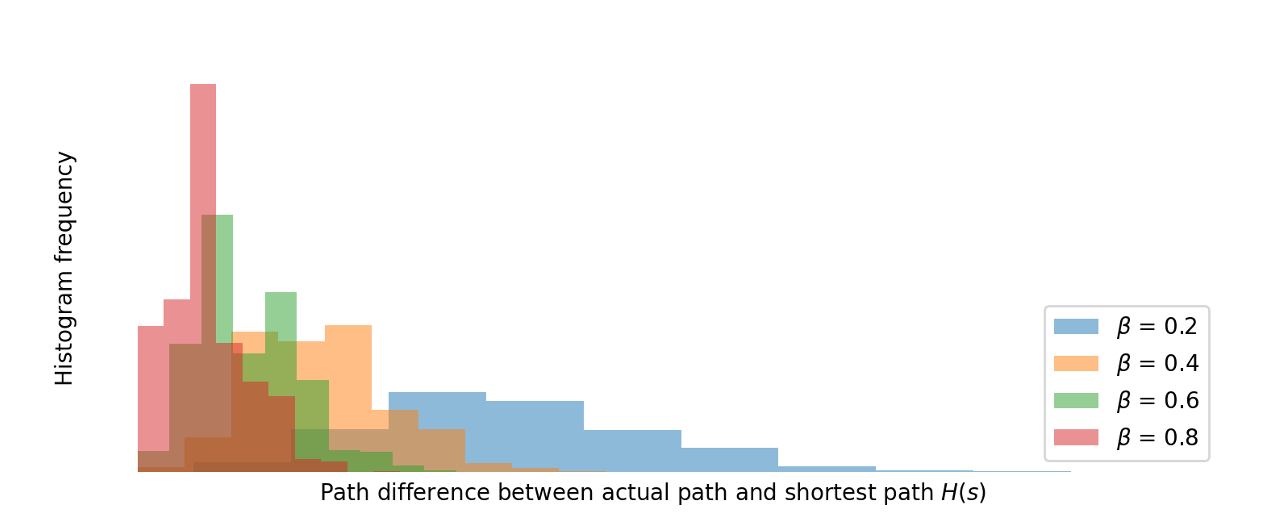
\includegraphics[width=\textwidth]{beta_vs_H.png}
\caption{Gibbs distribution with different parameter $\beta$}
\label{fig:beta}
\end{figure}

We designate the distribution of $H(s)$ to follow a Gibbs distribution. More commonly seen in statistical mechanics, Gibbs distribution gives the probability that a system will be in a certain state as a function of that state's energy and the temperature of the system \cite{}. We use a single parameter $\beta$, which measures the sinuosity of a network (the energy at a certain state). When $\beta=0$, the sampling distribution is uniform, and the resulting samples are more likely to have higher $H(s)$. When $\beta$ is large, the resulting samples are more likely to have lower $H(s)$ and are more efficient graphs. A Gibbs distribution has the following probability density function: \\
\[P_{\beta}\{s\} = [C(\beta)]^{-1} e^{-\beta H(s)}\]
As described in above, $\beta$ is a distribution parameter that measures the sinuosity of probability distribution, $H(s)$ is the network path difference calculated for each graph generated. $C(\beta)$ is a normalization coefficient. The spanning tree networks are generated following the simulated annealing methods on the basis of a stochastic Markov chain \cite{Aldous1987, Troutman1992,Seo2012}. \textcolor{blue}{Supporting information: describing the process and transition matrix etc.}

One way to sample spanning trees from a set of subgraphs of $G$ is to use a Monte Carlo Markov chain approach, where the probability of a spanning tree's occurrence follows a probability distribution of choice. In this case, a Gibbs distribution based Monte Carlo Markov chain algorithm used in Troutman and Karlinger \citeA{Troutman1992} is used to generate tree graphs, where the transition probabilities define on $H(s)$ and $\beta$. 

%The main parameter controlling network structure is the degree of network sinuosity. Each spanning tree takes an actual flow path to the outlet of the network, designated by the configuration of its directed edge. But on the grid, there is also the shortest path each node takes to the outlet of the network. This network path difference between the actual and shortest flow path is used as a main parameter to control the network structure.

The motivation for generating networks with different degrees of sinuosity is \textcolor{red}{so that we can differentiate the response of stormwater networks that share the same footprint but have different flow pathways/lengths. These different flow pathways can be encapsulated in a scenario of urban sprawl (i.e. low-density), assuming low and high density follows... High (sinuosity), low (more spreadout, direct pathways).} translate above-ground development patterns (e.g. urban sprawl versus high-density clusters) to underground infrastructure. Given the same acreage of land (i.e. the node size of the network), some communities are more tightly clustered and others are more spread out. The more clustered communities have lower degrees of sinuosity, because they take the nearly shortest paths to the network outlet. The actual flow paths existing in the communities with higher degrees of urban sprawl have higher degrees of sinuosity. 

We generate networks from a $n$-by-$n$ grid graph to reduce the dimensionality. 

Once the structure of the network is determined, we can place green infrastructure on the nodes of the network. The green infrastructure can be placed in the network by random assignment or by mean distance to the stormwater network outlet. 

\begin{figure}
 \noindent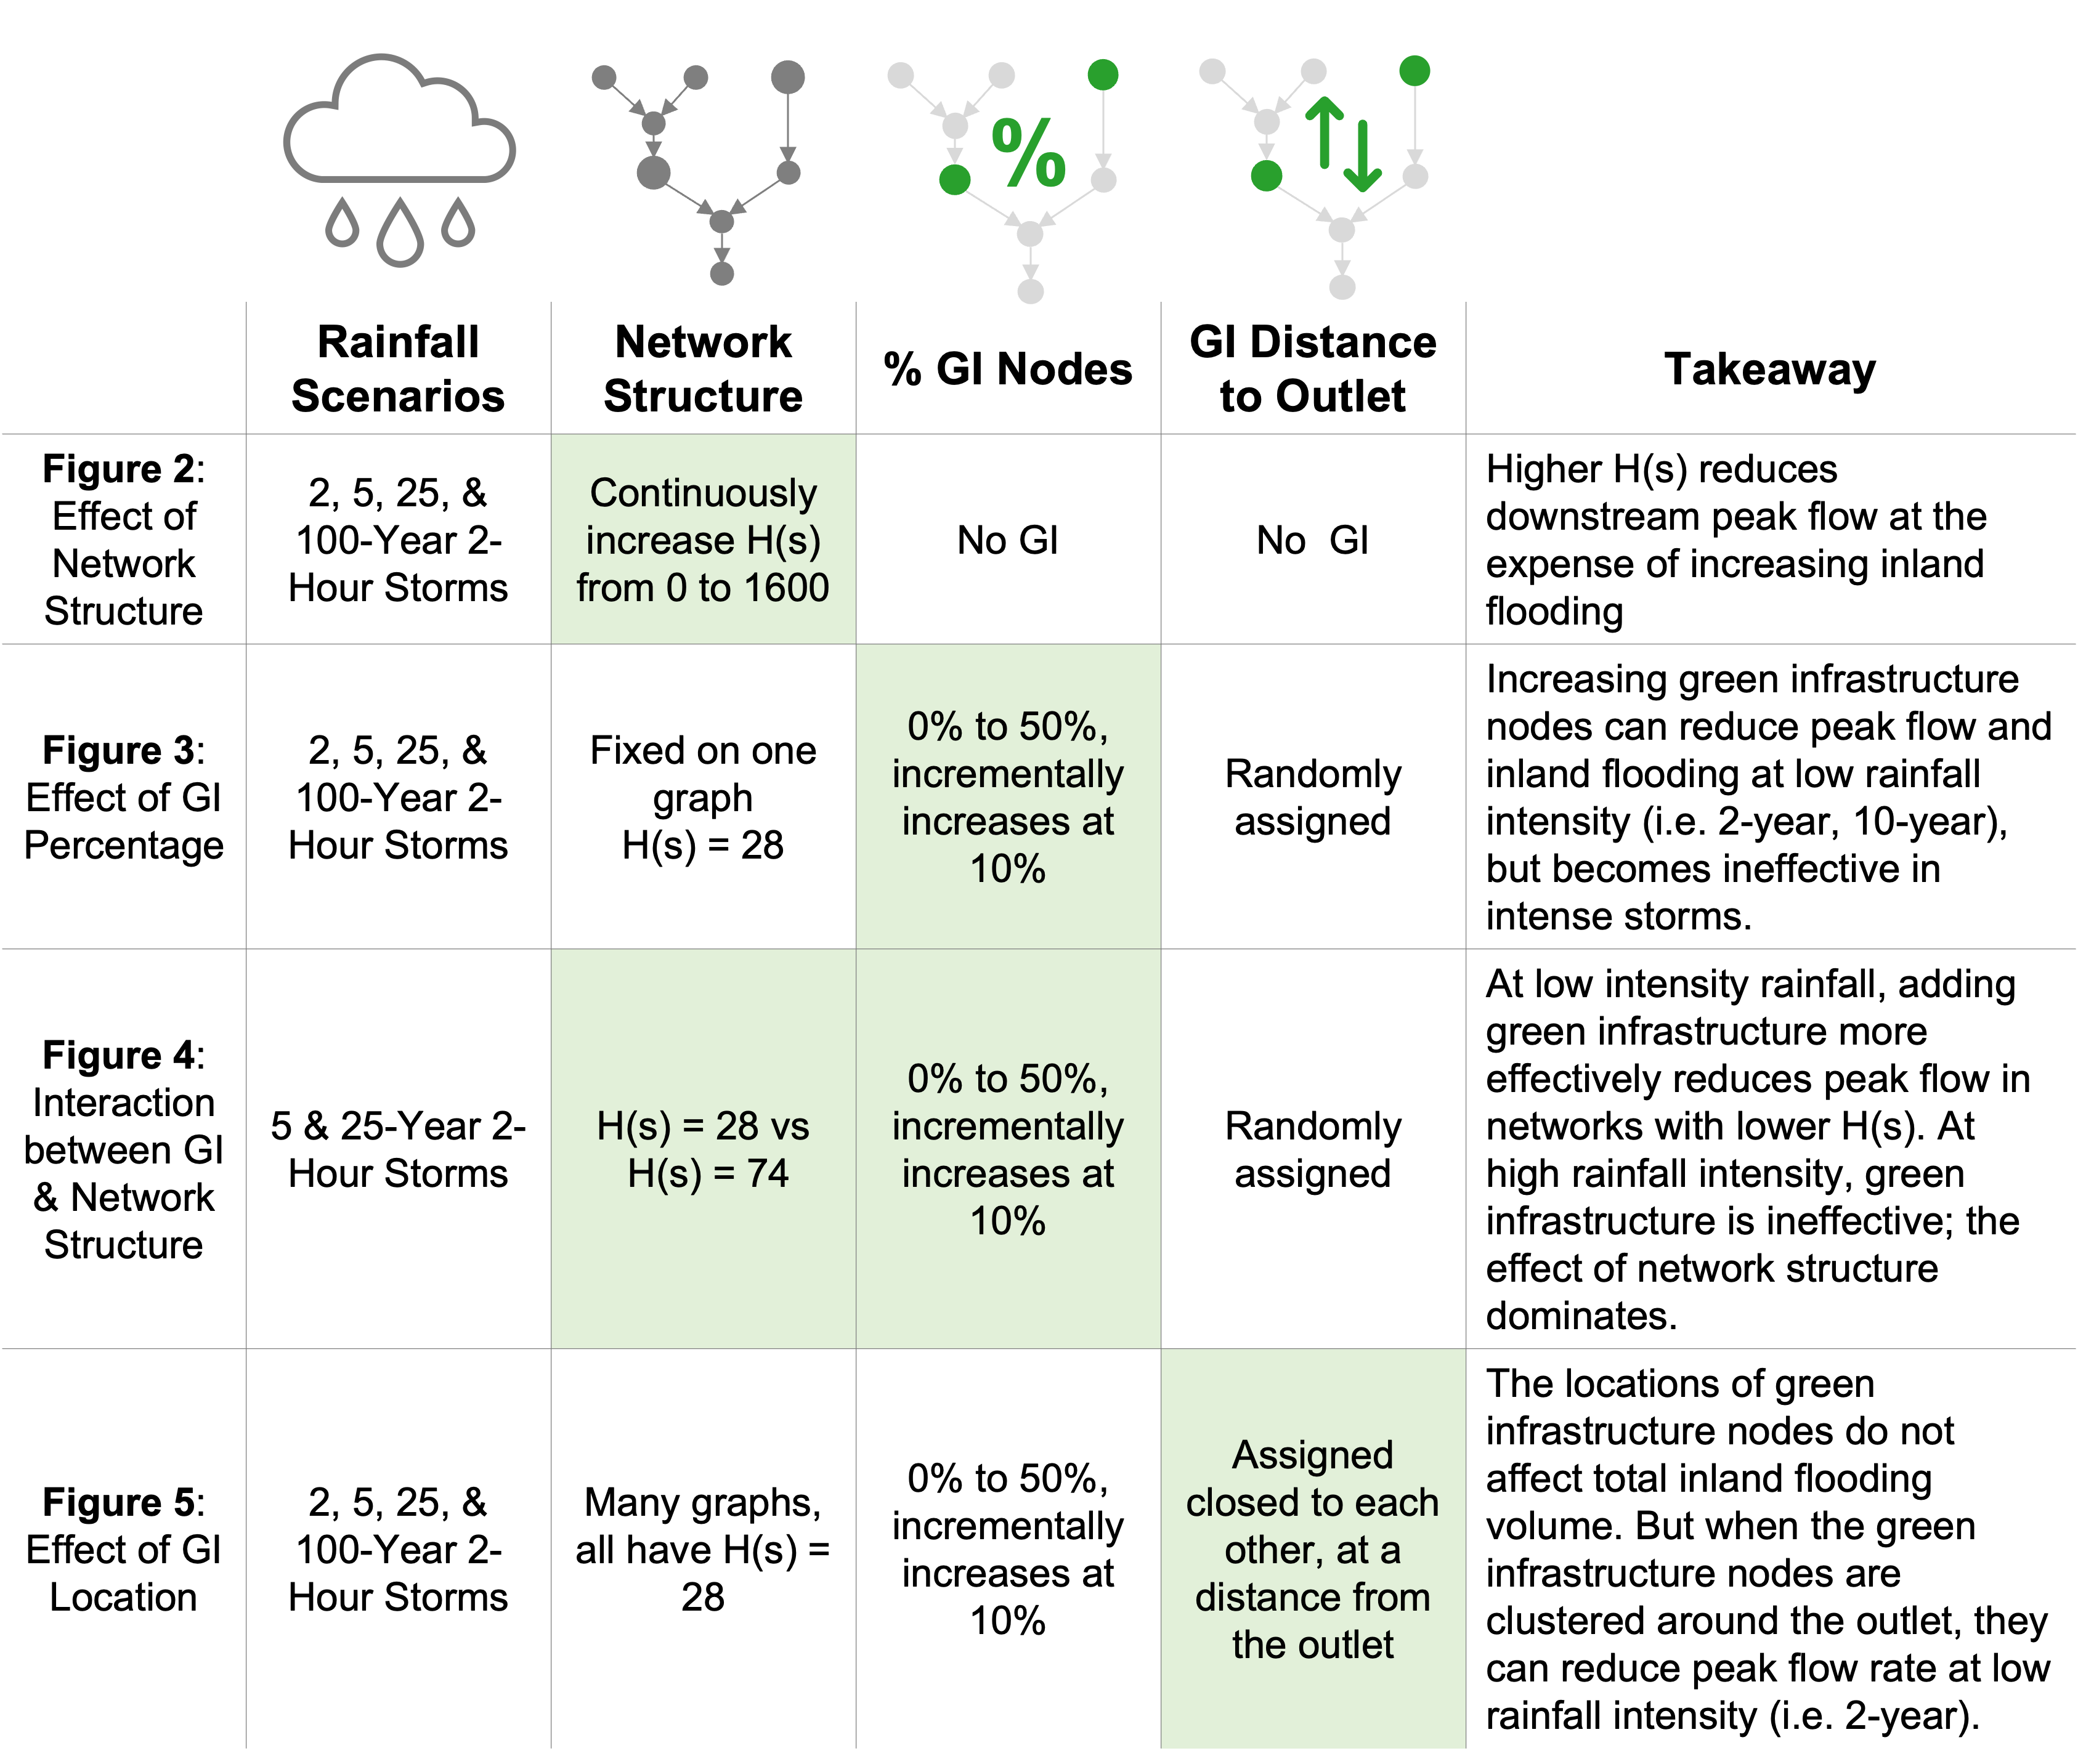
\includegraphics[width=\textwidth]{schema.png}
\caption{Pending caption}
 \label{fig:schema}
\end{figure}

\subsection{Green infrastructure and stormwater network design variable}
\textcolor{red}{Talk about theory, save implementation for later}
In this study, we generated graphs on an $n$-by-$n$ grid. For each simulated network, the network path difference $H(s)$ is calculated to represent the network structure, because we are comparing networks with fixed grids, and $H(s)$ is a more direct calculation of a graph's sinuosity than the normalized parameter $\beta$ for Gibbs distribution. Green infrastructure percentage ranges from 0 to 50\% at an increment of 10\%. The location of green infrastructure is calculated based on the nodes' distance to the network outlet. To study this effect, we created clusters of 10 green infrastructure nodes (10 \%) to reduce the large-variance effects arisen from a wide range of distances, and averaged the distances to outlet for each node in a cluster. (Why we do this cluster)

\begin{table}
 \caption{Network Design Attributes (SWMM Input)}
 \label{tab:SWMM}
 \centering
 \begin{tabular}{c l c c}
 \hline
Asset type & Attributes & Initial values & Exceptions \\
 \hline
& Relative elevation (ft) & 90 - 100 & 85 (outlet node) \\
& Subcatchment drainage area (acre) & 2 & $5\times 10^8$  (outlet node)\\
 & Manhole area (sqft) & 50 & $5\times 10^8$  (outlet node)\\
Nodes& Subcatchment impervious area (\%) & 60 & -- \\
& Subcatchment slope (\%) & 0.5 & -- \\
& Initial level	 (ft) & 0 & 1 (outlet node) \\
&Flood level (ft) & 10 & 0  (outlet node) \\
\hline
& GI/LID type & Bioretential Cell & -- \\
& Berm height (in) & 9 & -- \\
& Surface roughness (--) & 0.1 & -- \\
& Surface slope (\%) & 1.0 & -- \\
& Berm height (in) & 9 & -- \\
&Soil thickness	(ft) & 2 & -- \\
&Soil porosity (-) & 0.43 & --  \\ 
&Soil field capacity (-) & 0.4 & -- \\	
&Soil wilting point (-) & 0.18 & -- \\	
&Soil conductivity (in/hr) & 1.5 & -- \\	
&Soil conductivity slope (\%) & 40 & -- \\
&Soil suction head (in) & 3.5 & -- \\
& Storage thickness 	(in & 0 & --\\
&Storage void ratio (--) & 0.25 & -- \\	
&Storage seepage (in/hr) & 1.3 & -- \\	
&Potential ET loss (ft/day) &0.005  & --  \\	
&Rooting depth (ft) &1& -- \\	
\hline
&Design storm	& 10-year 24-hour & -- \\
&Slope & 0.008 & -- \\
Pipes &Manning’s n &0.01 & -- \\
&Length (ft) & 400 & (outlet pipe)\\
&Shape & Circular &  --\\
\hline
&Hydrographs & & \\
 \hline
 \end{tabular} \end{table}
 
  \begin{table}
 \caption{Rainfall Intensities of a Two-Hour Storm}
 \label{tab:rainfall}
 \centering
 \begin{tabular}{c c c}
 \hline
Return period & Total rainfall (inch) & 15-minute simulation (inch) \\
 \hline
2-Year & 1.69 & 0.211 \\
5-Year & 2.15 & 0.269 \\
10-Year & 2.59 & 0.324 \\
25-Year & 3.29 & 0.411 \\
100-Year & 4.55 & 0.569 \\
 \hline
 \end{tabular}
 \end{table}
 
\subsection{SWMM implementation}
We evaluated the performance of the green infrastructure network under two objectives: lowering peak flow rate at the stormwater network outlet, and reducing inland flooding volume upstream. The hydrological modeling was conducted using the Stormwater Management Model from Environmental Protection Agency (EPA-SWMM). The peak flow rate and inland flooding volume from SWMM output files were parsed and recorded. \textcolor{red}{(Supporting Information)} The fixed design attributes for the stormwater network itself and for the green infrastructure within the network are listed in Table~\ref{tab:SWMM}. 

We hypothesized that certain environmental variables may reduce green infrastructure's effectiveness. As a result, the SWMM model was run under five different two-hour rainfall scenarios, with return periods ranging from two years to 100 years. The two-hour storm was uniformly distributed to 15-minute intervals in the hyetographs as listed in Table~\ref{tab:rainfall}.

Directed edges in the network represent the stormwater pipes and their flow directions. Notably, the pipes in the network are sized using rational method with a 10-year 24-hour design storm. \textcolor{red}{Talk about sizing}

Nodes in the network represent access points in the stormwater network. \textcolor{red}{How do we determine the percentage of land cover distribution?}

Green infrastructure nodes. Parameters for green infrastructure \textcolor{red}{International Best Management Practice (BMP) Database}

 \begin{table}
 \caption{Summary of Simulation Set-up and Results}
 \label{tab:schema}
 \centering
 \begin{tabular}{p{1.8cm} | p{1.8cm}  p{1.8cm}  p{1.8cm}  p{1.8cm} | p{4cm}}
 \hline
Figure & Rainfall Scenarios & Network Structure & \% GI Nodes & GI Distance to Outlet & Takeaway \\
 \hline
Fig 1: Effect of network structure & 
2, 10, 25 \& 100-Year 2-Hour Storms & 
\textbf{$H(s)$ from 0 to 1600}& 
No GI & 
No GI & 
Higher $H(s)$ reduces downstream peak flow at the expense of increasing inland flooding \\ [0.5cm]

Fig 2: Effect of GI Percentage & 
2, 10, 25 \& 100-Year 2-Hour Storms & 
Fixed on one graph $H(s) = 28$ & 
\textbf{0\% to 50\%, incrementally increases at 10\%} & 
Randomly assigned & 
Increasing green infrastructure nodes can reduce peak flow and inland flooding at low rainfall intensity (i.e. 2-year, 10-year), but becomes ineffective in intense storms. \\ [0.5cm]

Fig 3: Interaction between GI \& Network Structure & 
5 \& 25-Year 2-Hour Storms & 
\textbf{$H(s) = 28$ vs $H(s) = 74$}& 
\textbf{0\% to 50\%, incrementally increases at 10\%} & 
Randomly assigned & 
At low intensity rainfall, adding green infrastructure more effectively reduces peak flow in networks with lower H(s). At high rainfall intensity, green infrastructure is ineffective; the effect of network structure dominates. \\ [0.5cm] 

Fig 4: Effect of GI Location & 
2, 10, 25 \& 100-Year 2-Hour Storms & 
Many graphs, all have $H(s) = 28$& 
0\% to 50\%, incrementally increases at 10\% & 
\textbf{Assigned closed to each other, at a distance from the outlet} & 
The locations of green infrastructure nodes do not affect total inland flooding volume. But when the green infrastructure nodes are clustered around the outlet, they can reduce peak flow rate at low rainfall intensity (i.e. 2-year). \\ [0.5cm] 
 \hline
 \end{tabular}
 \end{table}
 
\section{Results}
Based on the simulated stormwater network and SWMM results, we investigate three design variables that may affect green infrastructure's ability in reducing inland flooding and downstream peak flow under different rainfall intensities, ranging from two-year to 100-year storms. In general, we see that tradeoff exists between managing the two hydrological outcomes, and the effects of green infrastructure saturate at high rainfall intensity. In the sections below, we will present the results on the specific design parameters. 

Network structure can regulate hydrological outcomes, but tradeoff exists between managing different flow control objectives; a network cannot lower peak flow and flooding at the same time. Networks with higher $H(s)$ increase the total flow path and travel time of the network, hence they can effectively reduce the peak flow rate at stormwater network outlet as shown in Figure~\ref{fig:network_structure}. However, networks with higher $H(s)$ also increase inland flooding. Also due to the increasing travel time, these networks are less efficient in mitigating stormwater from upstream to downstream, especially when the event storm intensities exceed that of the design storm. 

The marginal hydrological benefits achieved by adding green infrastructure depend on the rainfall intensities and network structure. In a fixed network, increasing number or percentage of green infrastructure can reduce peak flow and inland flooding at low rainfall intensity (i.e. 2-year, 10-year), as shown in Figure~\ref{fig:GI_number}. However, at high rainfall intensity (i.e. 25-year, 100-year), the effect of additional green infrastructure saturated and the network structure $H(s)$ dominates the outcomes; although increasing percentage of green infrastructure can still reduce inland flooding volume, it can no longer reduce peak flow rate. The green infrastructure in the network transitions from a flood control measure to a flooding contributor \textcolor{red}{(Run this again and see why 25-year is like that? and combine the interaction with network structure).} Comparing different network structures, the network with lower $H(s)$ benefit $H(s)$ benefit more from additional green infrastructure in the network at lower rainfall intensity. 

The placement strategy of green infrastructure also depends on the targeted rainfall intensity and desired hydrological outcome. When placed closer to the outlet, green infrastructure can typically lower peak flow, but at the expense of slightly increasing inland flooding. The results, as shown in Figure~\ref{fig:distance}, also demonstrate that the peak flow reduction effects are more prominent under lower-rainfall intensity. The peak flow reduction of green infrastructure saturates at high rainfall intensity. 

 \begin{figure}
 \noindent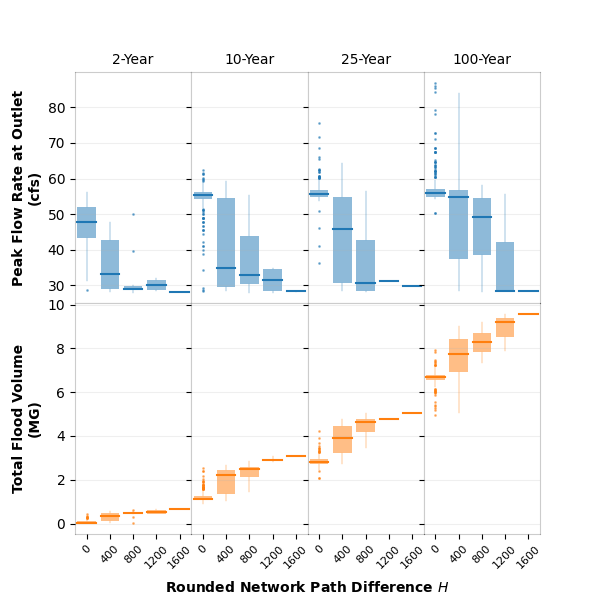
\includegraphics[width=\textwidth]{network_structure.png}
\caption{Effect of network structure: peak flow and inland flooding in networks with varying degrees of network path difference $H(s)$, under 2-year to 100-year two-hour storms. Generally, increasing $H(s)$ lowers peak flow rate, but it does so at the expense of increasing inland flooding. Network structure's effect on increasing inland flooding is more obvious in high-intensity storm.}
 \label{fig:network_structure}
\end{figure}

 \begin{figure}
 \noindent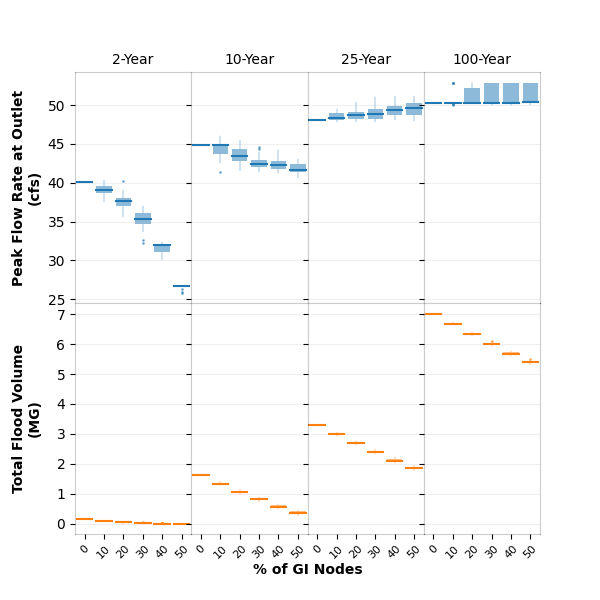
\includegraphics[width=\textwidth]{GI_number.png}
\caption{Effect of green infrastructure percentage: peak flow and inland flooding in networks with a fixed network and varying percentages of green infrastructure nodes, under 2-year to 100-year 2-hour storms. }
\label{fig:GI_number}
\end{figure}

 \begin{figure}
 \noindent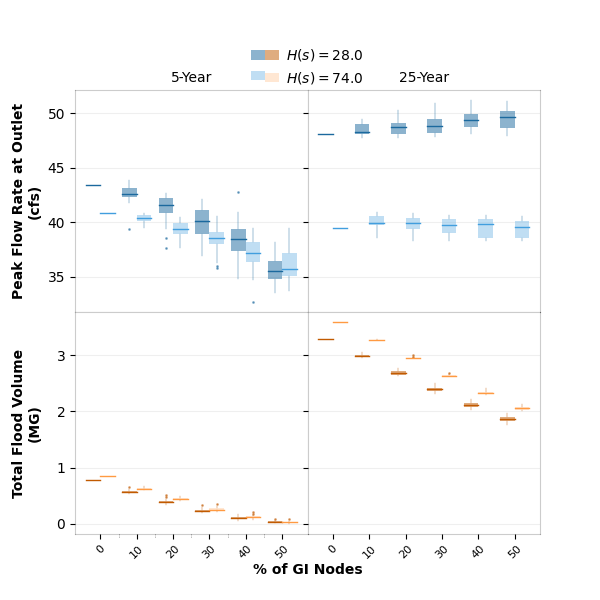
\includegraphics[width=\textwidth]{GI_network_interaction.png}
\caption{Interaction between green infrastructure and network structure: peak flow and inland flooding in networks with two fixed networks -- $H(s) = 28$ and $H(s) = 74$ -- and varying percentages of green infrastructure nodes, under 5-year and 25-year 2-hour storms.}
\label{fig:interaction}
\end{figure}

 \begin{figure}
 \noindent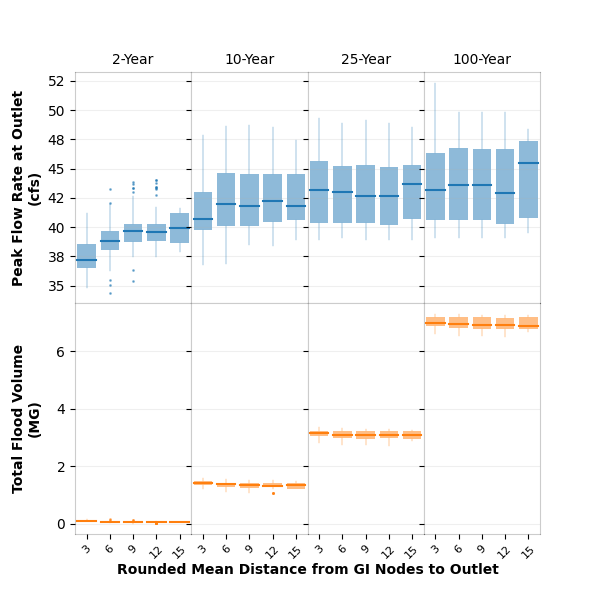
\includegraphics[width=\textwidth]{GI_placement28_new_rainfalls.png}
\caption{Effect of green infrastructure placement shown as the distance to the network outlet: peak flow and inland flooding in multiple networks with $H(s) = 28$ and varying placement of green infrastructure nodes, under 2-year to 100-year 2-hour storms. }
\label{fig:distance}
\end{figure}

\newpage
\section{Discussion} (Summarize then open up to the introductory questions again)
\textcolor{blue}{What does this mean for the design of network structure?}\\
\textcolor{blue}{What questions would need to be answered for this to be a useful tool for infrastructure planners?}\\
\textcolor{blue}{Does this line of work suggest that decentralized stormwater management is likely to be more effective at reducing flooding, as opposed to more centralized stormwater detention?}
\textcolor{red}{Have other studies address the spatial placement problem using SWMM? Are these surprising results (e.g. 5-10 references with GI performance under high rainfall intensity? City-wide rain garden adoption?) Network structures (e.g. maybe natural systems?) How novel is the finding or how well it fits into other studies? What are the limitations of the study (e.g. uncertainty related to parameter values, different types of green infrastructure)? What kind of new questions do we want to do in a new study?}\\

Appears to be the first study to combine the network structure with green infrastructure placement, where the network is quantified by its flow path instead of its topology. 

In this paper, we have shown that urban stormwater network and green infrastructure design can only effectively control water quantity under certain rainfall scenario. Tradeoff exists between managing different hydrological outcomes, and green infrastructure become ineffective under high rainfall intensity. Although there is no one-size-fits-all solution for green infrastructure implementation, refining the hydrological control objectives and understanding the network structure of the urban stormwater network will contribute to green infrastructure site selections at a watershed scale. 

The 100-node networks in this study were generated on a 10-by-10 grid. At this scale, our networks are large enough to capture the nuances in the competing hydrological outcomes and allow reasonably flexible re-configuration for scenario testing purposes, but these graphs are small comparing to any actual stormwater networks. More realistic reconstructions of stormwater networks require expansion of the network size and in-depth analyses of the real municipal stormwater network structure. However, these are non-trivial hurdles. Increasing the grid size will significantly increase the computational time to generate a graph. And spatial data for municipal stormwater networks have proven to be hard to access. 

Current literature on the effectiveness of green infrastructure focuses on either local-scale benefits, or specific configurations within a real-world stormwater network. As green infrastructure gets more attention as a valuable asset for climate adaption at a municipal level, the effectiveness of green infrastructure needs to be upscaled accordingly, and the underlying stormwater conveyance networks green infrastructure belongs to also needs to be evaluated. 

What is the missing gap for the next steps? 

(How does this fit in the larger research context? How does it contribute to the larger research?)

%Text here ===>>>


%%

%  Numbered lines in equations:
%  To add line numbers to lines in equations,
%  \begin{linenomath*}
%  \begin{equation}
%  \end{equation}
%  \end{linenomath*}



%% Enter Figures and Tables near as possible to where they are first mentioned:
%
% DO NOT USE \psfrag or \subfigure commands.
%
% Figure captions go below the figure.
% Table titles go above tables;  other caption information
%  should be placed in last line of the table, using
% \multicolumn2l{$^a$ This is a table note.}
%
%----------------
% EXAMPLE FIGURES
%
% \begin{figure}
% \includegraphics{example.png}
% \caption{caption}
% \end{figure}
%
% Giving latex a width will help it to scale the figure properly. A simple trick is to use \textwidth. Try this if large figures run off the side of the page.
% \begin{figure}
% \noindent\includegraphics[width=\textwidth]{anothersample.png}
%\caption{caption}
%\label{pngfiguresample}
%\end{figure}
%
%
% If you get an error about an unknown bounding box, try specifying the width and height of the figure with the natwidth and natheight options. This is common when trying to add a PDF figure without pdflatex.
% \begin{figure}
% \noindent\includegraphics[natwidth=800px,natheight=600px]{samplefigure.pdf}
%\caption{caption}
%\label{pdffiguresample}
%\end{figure}
%
%
% PDFLatex does not seem to be able to process EPS figures. You may want to try the epstopdf package.
%

%
% ---------------
% EXAMPLE TABLE
% Please do NOT include vertical lines in tables
% if the paper is accepted, Wiley will replace vertical lines with white space
% the CLS file modifies table padding and vertical lines may not display well
%
%% SIDEWAYS FIGURE and TABLE
% AGU prefers the use of {sidewaystable} over {landscapetable} as it causes fewer problems.
%
% \begin{sidewaysfigure}
% \includegraphics[width=20pc]{figsamp}
% \caption{caption here}
% \label{newfig}
% \end{sidewaysfigure}
%
%  \begin{sidewaystable}
%  \caption{Caption here}
% \label{tab:signif_gap_clos}
%  \begin{tabular}{ccc}
% one&two&three\\
% four&five&six
%  \end{tabular}
%  \end{sidewaystable}

%% If using numbered lines, please surround equations with \begin{linenomath*}...\end{linenomath*}
%\begin{linenomath*}
%\begin{equation}
%y|{f} \sim g(m, \sigma),
%\end{equation}
%\end{linenomath*}

%%% End of body of article

%%%%%%%%%%%%%%%%%%%%%%%%%%%%%%%%
%% Optional Appendix goes here
%
% The \appendix command resets counters and redefines section heads
%
% After typing \appendix
%
%\section{Here Is Appendix Title}
% will show
% A: Here Is Appendix Title
%
%\appendix
%\section{Here is a sample appendix}

%%%%%%%%%%%%%%%%%%%%%%%%%%%%%%%%%%%%%%%%%%%%%%%%%%%%%%%%%%%%%%%%
%
% Optional Glossary, Notation or Acronym section goes here:
%%%%%%%%%%%%%%
% Acronyms
   \begin{acronyms}
   \acro{GI}
   Green Infrastructure
   \acro{SWMM}
   Stormwater Management Model
   \end{acronyms}

%
%%%%%%%%%%%%%%
% Notation
%   \begin{notation}
%   \notation{$a+b$} Notation Definition here
%   \notation{$e=mc^2$}
%   Equation in German-born physicist Albert Einstein's theory of special
%  relativity that showed that the increased relativistic mass ($m$) of a
%  body comes from the energy of motion of the body—that is, its kinetic
%  energy ($E$)—divided by the speed of light squared ($c^2$).
%   \end{notation}




%%%%%%%%%%%%%%%%%%%%%%%%%%%%%%%%%%%%%%%%%%%%%%%%%%%%%%%%%%%%%%%%
%
%  ACKNOWLEDGMENTS
%
% The acknowledgments should list:
%
% 	All funding sources related to this work from all authors
%
% 	Any real or perceived financial conflicts of interests for any
%	author
%
% 	Other affiliations for any author that may be perceived as
% 	having a conflict of interest with respect to the results of this
% 	paper.
%
%   It is also the appropriate place to thank colleagues and other contributors.
%   AGU does not normally allow dedications.

%%%%%%%%%%%%%%%%%%%%%%%%%%%%%%%%%%%%%%%%%%%%%%%

\section*{Open Research}

%Open Research
% AGU requires an Availability Statement for the underlying data needed to understand, evaluate, and build upon the reported research at the time of peer review and publication.

%Additionally, authors should include an Availability Statement for the software that has a significant impact on the research. Details and templates are in the Availability Statement section of the Data & Software for Authors Guidance:
% https://www.agu.org/Publish-with-AGU/Publish/Author-Resources/Data-and-Software-for-Authors#availability

%For physical samples, use the IGSN persistent identifier, see the International Geo Sample Numbers section:
%https://www.agu.org/Publish-with-AGU/Publish/Author-Resources/Data-and-Software-for-Authors#IGSN
%%%%%%%%%%%%%%%%%%%%%%%%%%%%%%%%%%%%%%%%%%%%%%%

\acknowledgments
This section is optional. Include any Acknowledgments here.

%% ------------------------------------------------------------------------ %%
%% References and Citations

%%%%%%%%%%%%%%%%%%%%%%%%%%%%%%%%%%%%%%%%%%%%%%%
\bibliography{/Users/xchen/Documents/UMN_PhD/bibtex/Urban_Stormwater_Research}

% In the References section, cite the data/software described in the Availability Statement (this includes primary and processed data used for your research). For details on data/software citation as well as examples, see the Data & Software Citation section of the Data & Software for Authors guidance
% https://www.agu.org/Publish-with-AGU/Publish/Author-Resources/Data-and-Software-for-Authors#citation

%%%%%%%%%%%%%%%%%%%%%%%%%%%%%%%%%%%%%%%%%%%%%%%


%Reference citation instructions and examples:
%
% Please use ONLY \cite and \citeA for reference citations.
% \cite for parenthetical references
% ...as shown in recent studies (Simpson et al., 2019)
% \citeA for in-text citations
% ...Simpson et al. (2019) have shown...
%
%
%...as shown by \citeA{jskilby}.
%...as shown by \citeA{lewin76}, \citeA{carson86}, \citeA{bartoldy02}, and \citeA{rinaldi03}.
%...has been shown \cite{jskilbye}.
%...has been shown \cite{lewin76,carson86,bartoldy02,rinaldi03}.
%... \cite <i.e.>[]{lewin76,carson86,bartoldy02,rinaldi03}.
%...has been shown by \cite <e.g.,>[and others]{lewin76}.
%
% apacite uses < > for prenotes and [ ] for postnotes
% DO NOT use other cite commands (e.g., \citet, \citep, \citeyear, \citealp, etc.).
% \nocite is okay to use to add references from your Supporting Information
%



\end{document}



More Information and Advice:

%% ------------------------------------------------------------------------ %%
%
%  SECTION HEADS
%
%% ------------------------------------------------------------------------ %%

% Capitalize the first letter of each word (except for
% prepositions, conjunctions, and articles that are
% three or fewer letters).

% AGU follows standard outline style; therefore, there cannot be a section 1 without
% a section 2, or a section 2.3.1 without a section 2.3.2.
% Please make sure your section numbers are balanced.
% ---------------
% Level 1 head
%
% Use the \section{} command to identify level 1 heads;
% type the appropriate head wording between the curly
% brackets, as shown below.
%
%An example:
%\section{Level 1 Head: Introduction}
%
% ---------------
% Level 2 head
%
% Use the \subsection{} command to identify level 2 heads.
%An example:
%\subsection{Level 2 Head}
%
% ---------------
% Level 3 head
%
% Use the \subsubsection{} command to identify level 3 heads
%An example:
%\subsubsection{Level 3 Head}
%
%---------------
% Level 4 head
%
% Use the \subsubsubsection{} command to identify level 3 heads
% An example:
%\subsubsubsection{Level 4 Head} An example.
%
%% ------------------------------------------------------------------------ %%
%
%  IN-TEXT LISTS
%
%% ------------------------------------------------------------------------ %%
%
% Do not use bulleted lists; enumerated lists are okay.
% \begin{enumerate}
% \item
% \item
% \item
% \end{enumerate}
%
%% ------------------------------------------------------------------------ %%
%
%  EQUATIONS
%
%% ------------------------------------------------------------------------ %%

% Single-line equations are centered.
% Equation arrays will appear left-aligned.

Math coded inside display math mode \[ ...\]
 will not be numbered, e.g.,:
 \[ x^2=y^2 + z^2\]

 Math coded inside \begin{equation} and \end{equation} will
 be automatically numbered, e.g.,:
 \begin{equation}
 x^2=y^2 + z^2
 \end{equation}


% To create multiline equations, use the
% \begin{eqnarray} and \end{eqnarray} environment
% as demonstrated below.
\begin{eqnarray}
  x_{1} & = & (x - x_{0}) \cos \Theta \nonumber \\
        && + (y - y_{0}) \sin \Theta  \nonumber \\
  y_{1} & = & -(x - x_{0}) \sin \Theta \nonumber \\
        && + (y - y_{0}) \cos \Theta.
\end{eqnarray}

%If you don't want an equation number, use the star form:
%\begin{eqnarray*}...\end{eqnarray*}

% Break each line at a sign of operation
% (+, -, etc.) if possible, with the sign of operation
% on the new line.

% Indent second and subsequent lines to align with
% the first character following the equal sign on the
% first line.

% Use an \hspace{} command to insert horizontal space
% into your equation if necessary. Place an appropriate
% unit of measure between the curly braces, e.g.
% \hspace{1in}; you may have to experiment to achieve
% the correct amount of space.


%% ------------------------------------------------------------------------ %%
%
%  EQUATION NUMBERING: COUNTER
%
%% ------------------------------------------------------------------------ %%

% You may change equation numbering by resetting
% the equation counter or by explicitly numbering
% an equation.

% To explicitly number an equation, type \eqnum{}
% (with the desired number between the brackets)
% after the \begin{equation} or \begin{eqnarray}
% command.  The \eqnum{} command will affect only
% the equation it appears with; LaTeX will number
% any equations appearing later in the manuscript
% according to the equation counter.
%

% If you have a multiline equation that needs only
% one equation number, use a \nonumber command in
% front of the double backslashes (\\) as shown in
% the multiline equation above.

% If you are using line numbers, remember to surround
% equations with \begin{linenomath*}...\end{linenomath*}

%  To add line numbers to lines in equations:
%  \begin{linenomath*}
%  \begin{equation}
%  \end{equation}
%  \end{linenomath*}



